\documentclass[a4paper,11pt,oneside]{report}

%\usepackage[lmargin=2.5cm,rmargin=2.5cm]{geometry}

\usepackage{eucal}
\usepackage{hyperref}
% 
\addtolength{\hoffset}{-0.7cm}
\addtolength{\textwidth}{2.5cm}%1.6avant
\addtolength{\voffset}{-1.5cm}
\addtolength{\textheight}{2.5cm}
\usepackage{multirow}
%jusqu'ici
%avant il y avait ca
\usepackage{color}
\usepackage[all]{xy}
\usepackage[centertags]{amsmath}
\usepackage{latexsym}
\usepackage{stmaryrd}
%jusqu icib
\usepackage{amsfonts}
%\usepackage{xav}
%avant il y avait ca

\usepackage{amssymb}
\usepackage{amsthm}

\frenchspacing  \linespread{1.1}%1.5avant
\usepackage{fancyhdr}
\pagestyle{fancy}
\usepackage[dvips]{epsfig}

%jusqu ici

\usepackage{graphicx}
\usepackage{t1enc}

\usepackage[latin1]{inputenc}


\usepackage{amscd}
\usepackage{graphics}
\setlength{\unitlength}{1mm}

%%%%%%%%%%%%%%%%%%%%%%%%%%%%%%%%%%%%%%%%%%%%%%%%%%%%%%%%%%%%%%%%%%%%%%%%%%%%%%%%%%%%%%%%%%%%%%%%%%%%%%%%%%%%%%%%%%%%%%%%%%
%%%%%%%%%%%%%%%%%%%%%%%%%%%%%%%%%%%%%%%%%%%%%%%%%%%%%%%%%%%%%%%%%%%%%%%%%%%%%%%%%%%%%%%%%%%%%%%%%%%%%%%%%%%%%%%%%%%%%%%%%%%%?
%%%%%%%%%%%%%%%%%%%%%%%%%%%%%%%%%%%%%%%%%%%%%%%%%%%%%%%%%%%%%%%%%%%%%%%%%%%%%%%%%%%%%%%%%%%%%%%%%%%%%%%%%%%%%%%%%%%%%%%%%%%



%
% \setlength{\headheight}{14pt}  %%
% \setlength{\oddsidemargin}{0pt} %%{52pt} %%
% \setlength{\evensidemargin}{0pt}       %%{10pt} %%
% \setlength{\marginparwidth}     {72pt}%%{72pt}
% \pagestyle{headings}
% \linespread{1.13}
% \textheight 22cm
% \textwidth 18cm
% \hoffset -.9 cm
%  \voffset -0.9 cm
%  \def\dessous#1\sous#2{\mathrel{\mathop{\kern0pt#2}\limits_{#1}}}
% \normalbaselineskip=18pt
% \normalbaselines
%
% \parindent.5cm
% \parskip=5pt
%%%%%%%%%%%%%%%%%%%%%%%%%%%%%%%%%%%%%%%%%%%%%%%%%%%%%%%%%%%%%%%%%%%%%%%%%%%%%%%%%%%%%%%%%%%%%%%%%%%%%%%%%%%
%%%%%%%%%%%%%%%%%%%%%%%%%%%%%%%%%%%%%%%%%%%%%%%%%%%%%%%%%%%%%%%%%%%%%%%%%%%%%%%%%%%%%%%%%%%%%%%%%%%%%%%%%%%?
%%%%%%%%%%%%%%%%%%%%%%%%%%%%%%%%%%%%%%%%%%%%%%%%%%%%%%%%%%%%%%%%%%%%%%%%%%%%%%%%%%%%%%%%%%%%%%%%%%%%%%%%%%%%


%%%%%%%%%%%%%%%%%%  Sommaire   %%%%%%%%%%%%%%%%%%
%\usepackage[french]{minitoc}
\usepackage[french]{minitoc}
\setcounter{minitocdepth}{1}
\setcounter{tocdepth}{3}

%%%%%%%%%%%%%%%%%%%%%%%%%%%%%%%%%%%%%%%%%%%%%%%%%%%%%%

%\usepackage[english]{babel}
\usepackage[french]{babel}

\makeatletter
\newcommand{\thechapterwords}
{ \ifcase \thechapter\or Un\or Deux\or Trois\or Quatre\or
Cinq\or Six\or Sept \or Huit\or Neuf\or Dix\or Onze\fi}
\def\thickhrulefill{\leavevmode \leaders \hrule height 1ex \hfill \kern \z@}
\def\@makechapterhead#1{%
  %\vspace*{50\p@}%
  \vspace*{15\p@}%
  {\parindent \z@ \centering \reset@font
        \thickhrulefill\quad
        \scshape \@chapapp{} \thechapterwords
        \quad \thickhrulefill
        \par\nobreak
        \vspace*{15\p@}%
        \interlinepenalty\@M
        \hrule
        \vspace*{15\p@}%
        \Huge \bfseries #1\par\nobreak
        \par
        \vspace*{15\p@}%
        \hrule
    \vskip 60\p@
    %\vskip 100\p@
  }}
\def\@makeschapterhead#1{%
  %\vspace*{50\p@}%
  \vspace*{15\p@}%
  {\parindent \z@ \centering \reset@font
        \thickhrulefill
        \par\nobreak
        \vspace*{15\p@}%
        \interlinepenalty\@M
        \hrule
        \vspace*{15\p@}%
        \Huge \bfseries #1\par\nobreak
        \par
        \vspace*{15\p@}%
        \hrule
    \vskip 60\p@
    %\vskip 100\p@
  }}
  \def\@makechapterhead#1{%
  %\vspace*{50\p@}%
  \vspace*{15\p@}%
  {\parindent \z@ \centering \reset@font
        \thickhrulefill\quad
        \scshape \@chapapp{} \thechapterwords
        \quad \thickhrulefill
        \par\nobreak
        \vspace*{15\p@}%
        \interlinepenalty\@M
        \hrule
        \vspace*{15\p@}%
        \Huge \bfseries #1\par\nobreak
        \par
        \vspace*{15\p@}%
        \hrule
    \vskip 60\p@
    %\vskip 100\p@
    }}
  \frenchspacing \pagestyle{headings}
%%avant c etait \frenchspacing  \linespread{1.1}%1.5avant
%%d?finition des ent?tes
\usepackage{fancyhdr}
\pagestyle{fancy}

%%%%%%%%%%%%%%%%%%%%%%%   mes packages:
\usepackage{frcursive}
\usepackage{pifont}
\usepackage{algorithmic}
\usepackage{algorithm}
\floatname{algorithm}{Algorithme}
\renewcommand{\algorithmicrequire}{\textbf{Initialser}}
\renewcommand{\algorithmicensure}{\textbf{Etapes d'\'evaluation d'un sous probl\`eme}}
\renewcommand{\algorithmicwhile}{\textbf{Tant Que}}
\renewcommand{\algorithmicdo}{\textbf{Faire}}
\renewcommand{\algorithmicendwhile}{\textbf{Fin du Tant Que}}
\renewcommand{\algorithmicend}{\textbf{Fin}}
\renewcommand{\algorithmicif}{\textbf{Si}}
\renewcommand{\algorithmicendif}{\textbf{Fin du Si}}
\renewcommand{\algorithmicelse}{\textbf{Sinon}}
\renewcommand{\algorithmicelsif}{\textbf{Fin du Sinon}}
\renewcommand{\algorithmicthen}{\textbf{Alors}}
\renewcommand{\algorithmicfor}{\textbf{Pour}}
\renewcommand{\algorithmicforall}{\textbf{Pour tout}}
\renewcommand{\algorithmicto}{\textbf{\‘a}}
\renewcommand{\algorithmicendfor}{\textbf{Fin du Pour}}
\renewcommand{\algorithmicdo}{\textbf{Faire}}
\renewcommand{\algorithmicloop}{\textbf{boucler}}
\renewcommand{\algorithmicendloop}{\textbf{fin de la boucle}}
\renewcommand{\algorithmicrepeat}{\textbf{r\’ep\’eter}}
\renewcommand{\algorithmicuntil}{\textbf{jusqu’\‘a}}
\renewcommand{\algorithmicprint}{\textbf{afficher}}



%avant il y avait ca
 \usepackage[dvips]{epsfig}
%jusqu ici

% Ceci permet d?avoir les noms de chapitre et de section
% en minuscules
%avant il y avait ca
\renewcommand{\sectionmark}[1]{\markboth{#1}{}}
\renewcommand{\sectionmark}[1]{\markright{\thechapter\ #1}}


\renewcommand{\sectionmark}[1]{\markboth{#1}{}}
%\renewcommand{\chaptermark}[1]{\markboth{#1}{}}
%\renewcommand{\sectionmark}[1]{\markright{\thesection\ #1}}
\fancyhf{} % supprime les en-t?tes et pieds pr?d?finis
\fancyhead[L,R]{\bfseries\thepage}% Left Even, Right Odd
\fancyhead[L]{\bfseries\rightmark} % Left Odd
\fancyhead[R]{\bfseries\leftmark} % Right Even
\renewcommand{\headrulewidth}{1pt}% filet en haut de page
\addtolength{\headheight}{14pt} % espace pour le filet (avant on avait 1pt
\renewcommand{\footrulewidth}{1.5pt}% filet en bas de page
%\addtolength{\footheight}{0.5pt} % espace pour le filet en bas
\fancypagestyle{plain}{ % pages de tetes de chapitre
\fancyhead{} % supprime l'entete
%\fancyfoot{} %supprime le pied de page
\renewcommand{\headrulewidth}{0pt}
}
\newcommand{\clearemptydoublepage}{%
\newpage{\pagestyle{plain}\cleardoublepage}}

\rhead{\textbf{\thepage}}
\lhead{\textsl{\leftmark}}

%\fancyfoot[LE, RO]{\tiny \textbf{Bakary MANGA \copyright URMPM/IMSP 2008}}
\fancyfoot[L, RO]{\tiny \textbf{NGOM El hadji \copyright Universit\'e Cheikh Anta Diop de Dakar / 2015}}
\fancyfoot[LO]{\tiny \emph{\textbf{Les M\'eta-heuristiques en Optimisation}}}
%\fancyfoot[RE]{\tiny \textsl{Geometry }}

\rhead{\textbf{\thepage}}
\lhead{\textsl{\leftmark}}
\usepackage{newlfont}

\usepackage[active]{srcltx}
\hfuzz2pt
\newlength{\defbaselineskip}
\setlength{\defbaselineskip}{\baselineskip}
\newcommand{\setlinespacing}[1]%
           {\setlength{\baselineskip}{#1 \defbaselineskip}}
\newcommand{\doublespacing}{\setlength{\baselineskip}%
                           {1.5 \defbaselineskip}}
\newcommand{\singlespacing}{\setlength{\baselineskip}{\defbaselineskip}}

\newtheorem{remarque}{Remarque}[section]
\newenvironment{prof}[1][Preuve]{\textbf{#1.} }{\ \rule{0.5em}{0.5em}}
\theoremstyle{plain}
\newtheorem{lemme}{Lemme}[section]
\newtheorem{exercice}{Exercice}[section]
\newtheorem{proposition}{Proposition}[section]
\newtheorem{theoreme}{Th\'eor\`eme}[section]
\newtheorem{definition}{D\'efinition}[section]
\newtheorem{corollaire}{Corollaire}[section]
\newtheorem{notation}{Notation}[section]
\newtheorem{exemple}{Exemple}[section]
\newtheorem{propri\'et\'e}{Propri\'et\'e}[section]
\newtheorem{theodef}{Th\'eor\`eme et D\'efinition}[section]
\newtheorem{rappel}{Rappel}[section]


\newcommand{\Z}{\mathbb Z}
\newcommand{\R}{\mathbb R}
\newcommand{\C}{\mathbb C}
\newcommand{\N}{\mathbb N}
\newcommand{\F}{\mathbb F}
%\newcommand{\1}{1 \! \! {\rm I}}
\newcommand{\cc}{\mathcal{C}}
\newcommand{\A}{\mathcal{A}}
\newcommand{\X}{\mathcal{X}}
\newcommand{\I}{\mathcal{I}}
\newcommand{\el}{\mathcal{L}}
\newcommand{\G}{\mathcal{G}}
\newcommand{\B}{\mathcal{B}}
\newcommand{\f}{\mathcal{F}}
\newcommand{\E}{\mathcal{E}}
\newcommand{\D}{\mathcal{D}}
\newcommand{\m}{\mathfrak m}
\newcommand{\M}{\mathcal{M}}
\newcommand{\W}{\mathcal{W}}
\newcommand{\n}{\mathcal{N}}
\newcommand{\ho}{\hbox{\rm Hom}}
\newcommand{\Q}{l \! \! \! Q}
\newcommand{\0}{/ \! \! \! 0}
\newcommand{\s}{\mathfrak{s}}
\newcommand{\g}{\mathfrak g}
\newcommand{\h}{\mathfrak h}
\newcommand{\pd}{\partial}
%\newcommand{\u }{\mathfrak u}
\newcommand{\der}{\hbox{\rm der}}
\newcommand{\pder}{\hbox{\rm Pder}}
\newcommand{\paut}{\hbox{\rm Paut}}
\newcommand{\sspan}{\hbox{\rm span}}
\newcommand{\trace}{\hbox{\rm trace}}
\newcommand{\Ri}{\hbox{\rm Ri}}
\newcommand{\Sc}{\hbox{\rm Sc}}


%%%%%%%%%%%%%%%%%%%%%%%%%%%%%%%%%%%%Commandes redefinies%%%%%%%%%%%%%%%%%%%%%%%
\newcommand{\beq}{\begin{equation}}
\newcommand{\eeq}{\end{equation}}
\newcommand{\beqn}{\begin{eqnarray}}
\newcommand{\eeqn}{\end{eqnarray}}
\newcommand{\bpro}{\begin{proposition}}
\newcommand{\epro}{\end{proposition}}
\newcommand{\blem}{\begin{lemma}}
\newcommand{\elem}{\end{lemma}}
\newcommand{\bdfn}{\begin{definition}}
\newcommand{\edfn}{\end{definition}}
\newcommand{\bcor}{\begin{corollary}}
\newcommand{\ecor}{\end{corollary}}
\newcommand{\bthm}{\begin{theorem}}
\newcommand{\ethm}{\end{theorem}}
\newcommand{\bex}{\begin{example}}
\newcommand{\eex}{\end{example}}
\newcommand{\brmq}{\begin{remark}}
\newcommand{\ermq}{\end{remark}}
\newcommand{\benum}{\begin{enumerate}}
\newcommand{\eenum}{\end{enumerate}}
\newcommand{\bitem}{\begin{itemize}}
\newcommand{\eitem}{\end{itemize}}
\newcommand{\bexer}{\begin{exercise}}
\newcommand{\eexer}{\end{exercise}}
\newcommand{\bproof}{\begin{proof}}
\newcommand{\eproof}{\end{proof}}
\newcommand{\eprop}{\end{prop}}
\newcommand{\bprop}{\begin{prop}}
\theoremstyle{plain}
%\frenchspacing
\linespread{1}

%\usepackage[latin1]{inputenc}

%\usepackage[french]{babel}

\usepackage{graphicx}
\usepackage{t1enc}

%%%%%%%%%%%%%%%%%%%%%%%%%%%%%%%%%%%%%%%%%%%%%%%%%%%%%%%%%%%%%%%%%%%%%%%%%%%%%%%%%%%%%%%%
% 
%\title{Les Méta-heuristiques en Optimisation}
%\author{El Hadji NGOM}
%\date{\today}

%%%%%%%%%%%%%%%%%%%%%%%%%%%%%%%%%%%%%%%%%%%%%%%%%%%%%%%%%%%%%%%%%%%%%%%%%%%%%%%%%%%%%%%%

% \includeonly{introduction,chapitre1-varietes-differentielles,chapitre2-varietes-riemannienes,
% chapitre3-connexion,chapter4-action-groupes,
% conclusion,references,index}

\usepackage{makeidx}
%\makeindex

\begin{document}
%\maketitle
\dominitoc

\begin{titlepage}
\begin{center}

\includegraphics[height=2cm,width=2cm]{UcadLogo} \\ 
{\bf Universit\'e Cheikh Anta Diop de Dakar (UCAD)} \\

\includegraphics[height=2cm,width=2cm]{logo}

\vspace{0.2cm}
{\bf Facult\'e Sciences et Techniques (FST)}\\
\vspace{0.2cm}
{{\bf\it D\'epartements Math\'ematiques et Informatiques (DMI)\\}}
\end{center}

%{\bf Order $n^0$ : 43/2010}

\vspace{1.2cm}

\begin{center}

{\bf M\'emoire Master II \\
\vskip 0.2cm 

Option : Marh\'ematiques de la d\'ecision et Recherche op\'erationnelle\\}

\vspace{1.5cm}
{\bf Titre :\\}
{\Large\bf Les M\'etaheuristiques en Optimisation\\ }
\vspace{0.5cm}
Par :

\vspace{1cm}

NGOM El hadji\footnote{UCAD-AIMS-SENGAL}\\

\vspace{1cm}

Jury :\\
\end{center}
\begin{tabular}{lcl}
Pr\'esident  &-& {\bf  Prof.       }\\
           & &                                                                            \\
Membres    & & {\bf Prof.            }\\             
           & & {\bf Prof.            } \\ 
           & & {\bf Prof.            }  \\
           & &                                                                             \\
Superviseurs &-& {\bf Prof. Salimata Gu\`eye Diagne (UCAD)   }      \\
            &-& {\bf Prof. Youssou GNINGUE Universit\'e Laurentiane (Canada)}
\end{tabular}

\vspace{1cm}

\begin{center}
{\bf Soutenue le $.....$}
\end{center}

\end{titlepage}
\pagenumbering{roman}


\chapter*{D\'edicaces}
\addstarredchapter{D\'edicaces}






\chapter*{Remerciements}
\addstarredchapter{Remerciements}




\chapter*{R\'esum\'e}
\addstarredchapter{R\'esum\'e}






\chapter*{Abstract}
\addstarredchapter{Abstract}





\tableofcontents
\listoffigures
\listoftables


\chapter*{Introduction g\'en\'erale}
\addstarredchapter{Introduction g\'en\'erale}
\fancyhead[L]{Introduction g\'en\'erale}
\pagenumbering{arabic}

L'optimisation est un concet bien naturel dans la vie courante: devant un probl\`eme en pr\'esence de plusieurs solutions possibles, tout individu
coisit ( en g\'en\'eal) une solution qualifi\'ee de ``meilleur''.\\
Les m\'ethodes \'exactes des problmes d'optimisation (combinatoire) permettent d'obtenir une solution dont l'optmalit\'e est garantie ou assur\'ee, 
dans certaines situations, on peut cependant chercher des solutions de bonne qualit\'e, sans garantie d'optimalit\'e mais avec un temps beaucoup 
consid\'erablement r\'eduit. Pour cela, on applique des m\'ethodes appel\'es  {\bf m\'etaheuristiques}  (ce mot vient du grec {\it meta} qui signifie 
litt\'eralement "au d\'ela" mais '{\it \'a un plus haut niveau}' dans ce contexte), adapt\'ees \'a chaque probl\'eme trait\'e, avec seulement
l'inconv\'enient de ne 
pas disposer en retour d'aucune information sur la qualit\'e de la solution obtenue. Les heuristiques comme les m\'etaheuristiques exploitent
generalement des
 processus al\'eatoires dans l'exploration de l'espace de recherche pour faire face \'a l'explosion combinatoire engendr\'ee par l'utilsation des methodes \'exactes. 
 Reposant sur une base stochastique, les m\'etaheuristiques sont plus souvent iteratives, ainsi le meme processus de recherche est rep\'et\'e lors de la r\'esolution.
 Les m\'etaheuristiques acqui\`erent une grande avantage par leur capacit\'e d'\'eviter les minima locaux en admettant des d\'egradations de la fonction objectve au
 cours de la progression.\\
 Grace \`a l'optimisation lineaire en nombres entiers, la discipline occupe une place capitale en mathematique d\'ecisionnaire, en recherche opreationnelle et en informatique.
 Des nombreuses applications peuvent \^etre mod\'elis\'ees sous la forme de probl\`eme d'optimisation en nombres entiers telles que le voyageur de commerce, le probl\`eme
 de coloration de graphe, les proble\`emes de localisation etc.
 En g\'en\'eral, on appelle programmation math\'ematique la recherche de l'optimum d'une fonction de plusieurs variables li\'ees entre elles
  par des contraintes (sous formes'\'egalit\'e ou d'in\'egalit\'e). En particulier voici la forme standard d'une programmation lin\'eaire:
 $$
    \left\{ 
        \begin{array}{c}
         \max  Z(x) \\
         s.c.\\
         H_i(x) \leq \alpha_i   \\
         x \in S \subset \mathbb{R}^n
        \end{array}
     \right.
     \hspace{1cm}
    \left\{ 
        \begin{array}{c}
         \min  Z(x) \\
         s.c.\\
         H_i(x) \geq \alpha_i  \\
         x \in S \subset \mathbb{R}^n
        \end{array}
     \right.  
 $$
 $$ i \in \{ 1, 2 , \hdots, m\}$$
Ici le vecteur $x\in \mathbb{Z}^n $ a pour composantes $x_1, x_2, \hdots, x_m$ qui les inconnues du probl\`eme.
La fonction $Z$ est la fonction objectif ( on dit parfois aussi: fonction \'economique) et l'ensemble des conditions: $H_i(x) \leq \alpha_i $ ou 
$H_i(x) \geq \alpha_i $ avec $i\in \{1,2,\hdots,m\}$ et $x \in S$ sont les contraintes du probl\`eme. 
%%%%%%%%%%%%%%%%%%%%%%%%%%%%%%%%%%%%%%%%%%%%%%%%%%%%%%%%%%%%%%%%%%%%%%%
%%%%%%%%%%%%%%%%%%%%%%%%%%%%%%%%%%%%%%%%%%%%%%%%%%%%%%%%%%%%%%%%%%%%%%%
\chapter{Les m\'ethodes de r\'esolution exactes et heuristiques}
%\minitoc
\section{Introduction}
R\'esoudre un probl\`eme d'optimisation lin\'eaire en nombres entiers consiste \`a chercher la meilleure solution possible pour ce probl\`eme, 
d\'efinie comme la solution globabalement optimale ou un optimum global. La r\'esolution de ces probl\`emes dits \'egalement combinatoires est
souvent assez d\'elicate puisque le nombre fini de solutions r\'ealisables cro\^it consi\'erablement avec la taille du probl\`eme, ainsi que sa 
complexit\'e. Cette remarque a pouss\'e les chercheurs \`a d\'evelopper de nombreuses m\'ethodes de r\'esolution aussi bien qu'en Recherche op\'erqtioonelle
(RO) qu'en intelligence artificielle (IA).\\
Dans la section suivante, nous allons d'abord d\'efinir les notions de complexit\'e quant aux probl\`emes d'optmisation combinatoire.
%%%%%%%%%%%%%%%%%%%%%%%%%%%%%%%%%%%%%%%%%%%%%%%%%%%%%%%%%%%%%%%%%%%%%%%%%%%%%%%%%%%%%%%%%%%%%%%%%%%%%%%%%%%%%%%%%%%%%%%%%%%
%%%%%%%%%%%%%%%%%%%%%%%%%%%%%%%%%%%%%%%%%%%%%%%%%%%%%%%%%%%%%%%%%%%%%%%%%%%%%%%%%%%%%%%%%%%%%%%%%%%%%%%%%%%%%%%%%%%%%%%%
\section{Notions de compl\'exit\'e}
Avant de passer \`a un bref rappel sur les differntes m\'ethodes de r\'esolution exactes et heuristiques des probl\`emes d'optimisation
lin\'eaires en nombres entiers, nous introduisons quelques d\'efinitions et notions sur la complexit\'e des ces derniers \`a savoir les
PLNE.\\ La th\'eorie de la complexit\'e des algorithmes, n\'ee \`a la suite des travaux d'Emonds puis Cook et karp, a justement pour objet
 de lier le nombre de calculs \'effectu\'es lors de la r\'esolution d'un probl\`eme au moyen d'un algorithme donn\'e \`a la taille des 
 donn\'ees de ce probl\`eme. Nous ne ferons pas diff\'erence entre algorithme et programme.\\
 En g\'en\'eral, le temps d'\'excution est le facteur majeur qui d\'etermine l'\'efficacit\'e d'un algorithme, alors la complexit\'e en temps 
 d'un algorithme est le nombre d'instructions n\'ecessaires (affectation, comparaison, op\'erations alg\'ebriques , lecture et \'ecriture,
 etc) que comprend cet algorithme pour une r\'esolution d'un probl\`eme quelconque.
\begin{definition}
 Une fonction $f(n)$ est $O(g(n))$ ou $(f(n)$ est de complexit\'e $g(n))$ s'il existe un r\'eel $c>0$ et un entier positif $n_0$ tels que
 pour tout $n>n_0$ on a $|f(n)| \leq c.g(n)$.
\end{definition}
%%%%%%%%%%%%%%%%%%%%%%%%%%%%%%%%%%%%%%%%%%%%%%%%%%%%%%%%%%%%%%%%%%%%%%%%%%%%%%%%%%%%%%%%%%%%%%%%%%%%%%%%%%%%%%%%%%%%%%%%%%%%%%%%%%%
\begin{definition}
 Un algorihme en temps polynomial est un algorithme dont le temps de la complexit\'e est en $O(p(n))$, o\`u $p$ est une fonction polynomiale
  et $n$ la taille de l'instance ( ou sa longueur d'entr\'ee).\\
 Si $k$ est le d\'egr\'e de ce polynome en $n$, le probl\`eme correspondant est dit \^etre r\'esoluble en $O(n^k)$ et appartient \`a la classe $P$. 
 La connexit\'e d'un grphe est un example de probl\`eme polynomial de classe $P$.
 \end{definition}
%%%%%%%%%%%%%%%%%%%%%%%%%%%%%%%%%%%%%%%%%%%%%%%%%%%%%%%%%%%%%%%%%%%%%%%%%%%%%%%%%%%%%%%%%%%%%%%%%%%%%%%%%%%%%%%%%%%%%%%%%%%%%%%%%%%%%%%%%%%%%%
\begin{definition}
 La classe {\bf NP} contient l'ensemble des probl\`emes de d\'ecision qui peuvent \^etre d\'ecid\'es sur une machine non d\'eterministe en temps polynomial.
 C'est la classe des probl\`emes qui admettent un algorihme en temps polynomial capable de tester la validit\'e d'une solution du probl\`eme.
 Intuitivement, les probl\`emes de cette classe sont les probl\`emes qui peuvent \^etre r\'esolus en \'enumerant l'ensemble des solutions possibles et
  les tester \`a l'aide d'un algorihme polynomial.
 \end{definition}
%%%%%%%%%%%%%%%%%%%%%%%%%%%%%%%%%%%%%%%%%%%%%%%%%%%%%%%%%%%%%%%%%%%%%%%%%%%%%%%%%%%%%%%%%%%%%%%%%%%%%%%%%%%%%%%%%%%%%%%%%%%%%%%%%%%%%%%%%%%%%%%%%%%
\begin{definition}
 On dit qu'un probl\`eme de recherche $P_1$ se r\'eduit polynomialement \`a un probl\`eme de recherche $P_2$ par r\'eduction de Turing s'il \'existe
  un algorihme $A_1$ pour r\'esoudre $P_1$ en utilisant comme sous programme un algorithme $A_2$ r\'esolvant $P_2$, de telle sorte que la complexit\'e
  $A_1$ est polynomiale, quand on \'evalue chaque appel de $A_2$ par une constante.
\end{definition}
%%%%%%%%%%%%%%%%%%%%%%%%%%%%%%%%%%%%%%%%%%%%%%%%%%%%%%%%%%%%%%%%%%%%%%%%%%%%%%%%%%%%%%%%%%%%%%%%%%%%%%%%%%%%%%%%%%%%%%%%%%%%%%%%%%%%%%%%%%%%%%%%%%%%
\begin{definition}[La classe {\bf NP-Complet}]
 Parmi l'ensemble des porbl\`eme des probl\`emes appartenant \`a {\bf NP}, il \'existe un sous ensemble qui contient les probl\`emes les plus difficiles: 
 on les appelle les probl\`emes {\bf NP-Complets}. Un probl\`eme de classe {\bf NP-Complet} poss\`ede la propri\'et\'e que tous les probl\`emes {\bf NP} lui
 sont r\'eductibles. Si on trouve un algorithme polynomial \`a un probl\`eme {\bf NP-Complet}, on trouve alors automatiquement une r\'esolution polynomiale
  de tous les probl\`emes {\bf NP} de la classe {\bf NP}.
\end{definition}
%%%%%%%%%%%%%%%%%%%%%%%%%%%%%%%%%%%%%%%%%%%%%%%%%%%%%%%%%%%%%%%%%%%%%%%%%%%%%%%%%%%%%%%%%%%%%%%%%%%%%%%%%%%%%%%%%%%%%%%%%%%%%%%%%%%%%%%%%%%%%%%%%%%%%%%%%%%
\begin{definition}[La classe {\bf NP-difficile}]
 Un probl\`eme est {\bf NP-difficile} s'il est plus difficile qu'un probl\`eme {\bf NP-Complet}, c'est-\`a-dire 
 s'il \'existe un probl\`eme {\bf NP-Complet} se r\'eduisant \`a ce probl\`eme par une r\'eduction de Turing.
\end{definition}
Nous allons passer \`a la description des principales m\'ethodes de r\'esolution exactes des probl\`emes d'optimisation combinatoire.
%%%%%%%%%%%%%%%%%%%%%%%%%%%%%%%%%%%%%%%%%%%%%%%%%%%%%%%%%%%%%%%%%%%%%%%%%%%%%%%%%%%%%%%%%%%%%%%%%%%%%%%%%%%%%%%%%%%%%%%%%%%%%%
%%%%%%%%%%%%%%%%%%%%%%%%%%%%%%%%%%%%%%%%%%%%%%%%%%%%%%%%%%%%%%%%%%%%%%%%%%%%%%%%%%%%%%%%%%%%%%%%%%%%%%%%%%%%%%%%%%%%%%%%%%%%%%%
\section{Les m\'ethodes exactes}
 Nous allons pr\'esenter d'abord quelconques m\'ethodes de la classe des algorithmes complets ou exactes, ces m\'ethdes donnent une garantie de trouver la
 solution optimale pour une instance de taille finie dans un temps limit\'e et de prouver son optimalit\'e [\ref{Schrijver}].
\subsection{La m\'ethode du Simplexe}\label{simplexe}
 Parmi ces m\'ethodes, on peut remarquer l'algorihme du simplexe qui permet d'obtenir la solution optimale d'un probl\'eme d'optimisation en parcourant la 
 fermeture convexe de l'ensemble de recherche. Son avantage c'est qu'il permet de r\'esoudre un grand nombre de probl\`emes rapidement.\\\vspace{0.4cm}
 Voici la d\'efinition donn\'ee par {\bf Wikip\'edia, (consult\'e le 25/12/2015)}:\\
   ``{\it L'algorithme du simplexe est un algorithme de r\'esolution des probl\`emes d'optimisation lin\'eaire. Il a \'et\'e introduit par George Dantzig
 \`a partir de 1947. C'est probablement le premier algorithme permettant de minimiser une fonction sur un ensemble d\'efini par des in\'egalit\'es. 
De ce fait, il a beaucoup contribu\'e au d\'emarrage de l'optimisation num\'erique. L'algorithme du simplexe a longtemps \'et\'e la m\'ethode la plus utilis\'ee
 pour r\'esoudre les probl\'emes d'optimisation lin\'eaire. Depuis les ann\'ees 1985-90, il est concurrenc\'e par les m\'ethodes de points int\'erieurs, mais garde 
 une place de choix dans certaines circonstances (en particulier si l'on a une id\'ee des contraintes d'in\'egalit\'e actives en la solution)}''.
 \vspace{0.4cm}
 
                                                                                  
 Cependant, l'algorihme du simplexe qui est bien entendu valable pour tout probl\`eme, il n'est n\'ecessairement le plus efficace pour traiter des
 probl\`emes dont l'ensemble des contraintes pr\'esente certaines particularit\'es (comme l'int\'egrit\'e de la solution).
%%%%%%%%%%%%%%%%%%%%%%%%%%%%%%%%%%%%%%%%%%%%%%%%%%%%%%%%%%%%%%%%%%%%%%%%%%%%%%%%%%%%%%%%%%%%%%%%%%%%%%%%%%%%%%%%%%%%%%%%%%%%%%%%%%%%%%%%%%%%%%%%
%%%%%%%%%%%%%%%%%%%%%%%%%%%%%%%%%%%%%%%%%%%%%%%%%%%%%%%%%%%%%%%%%%%%%%%%%%%%%%%%%%%%%%%%%%%%%%%%%%%%%%%%%%%%%%%%%%%%%%%%%%%%%%%%%%%%%%%%%%%%%%%%
\subsection{La M\'ethode de S\'eparation et d'Evauation}
 L'algorihme de s\'eparation et d'\'evaluation, connu sous l'appellation anglaise {\bf Branch and Bound (B\&B)}, est l'une des methodes les plus
 connues pour r\'esolution de probl\`emes d'optimisation combinatoires NP-Complets comme {\bf le probl\`eme de sac \`a dos}\footnote{Knapsack Problem 
  (KP)ou probl\`eme de sac \`a dos est un probl\`eme simple et classique d'optimisation combinatoire appartenant \`a la classe NP-Complet.}.
 Elle repose sur une m\'ethode arborescente de recherche d'une solution optimale par s\'eparations et \'evaluations, repr\'esentant les \'etats 
 solutions par un arbre d'\'etats, avec des noeuds, et des feuilles.\\
  Le branch and bound est bas\'e sur tois axes principaux:
  \begin{description}
   \item[\ding{46}] {\bf l'\'evaluation},
   \item[\ding{46}] {\bf la s\'eparation},
   \item[\ding{46}] {\bf la strat\'egie de parcours}.
  \end{description}
 \ding{43} {\bf L'\'evalution}:
  \begin{description}
  \item l'\'evaluation permet de rediure l'espace en \'eliminant quelques sous ensembles qui ne contiennent pas la solution optimale. L'objectif est d'essayer
   d'\'evaluer l'int\'er\^et de l'exploration d'un sous ensemble de l'arborescence. Le branch and bround utilise une \'elimination de branches dans l'
   arborescence de recherche de la mani\`ere suivante: la recherche d'une solution de co\^ut minimal, consiste \`a m\'emoriser la solution la moins
   co\^uteuse rencontr\'ee pendant l'exploration, et \`a comparer le co\^ut de chaque noeud parcouru \`a celui de la meilleure solution. Si le co\^ut du
   noeud consid\'er\'e est sup\'ereiur au meilleur co\^ut, on arr\^et l'exploration de la branche et toutes les solutions de cette branche seront 
   n\'ecssairement de cou\^ut plus \'elev\'e que la solution d\'eja trouc\'ee. 
  \end{description}
 \ding{43} {\bf La s\'eparation}:
 \begin{description}
 \item la s\'eparation consiste \`a diviser le probl\`eme en sous probl\`emes et en gardant la meilleure solution trouv\'ee, on est assur\'e d'avoir r\'esolu
  le probl\`eme inintial. cela revient \`a construire un arbre permettant d'\'enumerer toutes les solutions. L'ensemble des noeuds de l'arbre qu'il reste
  encore parcourir comme \'etant susceptibles de contenir une solution optimale, c'esr-\`a-dire encore \`a divser, est appel\'e ensemble des noeuds actifs.\\
  La proc\'edure de s\'eparation s'arr\^ete losrqu'une des conditions suivantes est v\'erif\'ee:
  \begin{description}
   \item[\ding{51}] on recoonait la meilleure solution de l'ensemble,
   \item[\ding{51}] on reconnait une solution meilleure que toutes celles de l'ensemble,
   \item[\ding{51}] on sait que l'ensemble ne cotient aucune soolution admissible.
  \end{description}
 \end{description}
 \ding{43} {\bf La strat\'egie de parcours}:
 \begin{description}
  \item[\ding{247}] {\bf La largeur d'abord:} cette strat\'egie favorise les sommets les plus proches de la racine en faisant moins de s\'eparations du probl\`eme 
  initial. Elle est moins efficace que les deux qui suivent, 
  \item[\ding{247}] {\bf La profonduer d'adord:} cette strat\'egie avantage les sommets les plus \'eloign\'es de la racine ( de profondeur plus \'elev\'ee) en applicant
   plus de s\'eparations au probl\`eme initial. Cette voie m\`ene rapidement \`a une solution optimale en \'economisant la m\'emoire,
  \item[\ding{247}] {\bf La meilleur d'abord:} cette strat\'egie consiste \`a exploere les sous-probl\`emes poss\'edant la meilleure borne. Elle permet aussi d'\'eviter l'exploration
   de tous les sous-probl\`emes qui poss\`edent une mauvaise \'evaluation par rapport \`a la valeur optimale. Elle dirige \'egalement la recherche l\`a o\`u
    la probabilit\'e de trouver une meilleure solution est plus forte.
 \end{description}

%%%%%%%%%%%%%%%     SCHEMA ILLUSTRATIF DE LA METHODE
 \begin{cursive} 
  {\bf Repr\'esentation graphique de la d\'ecomposition par B\&B appliqu\'ee au KP:}
 \end{cursive}
\underline{\bfseries Formulation math\'ematique du KP:} Dans ce cas, nous avons un sac \`a dos de maximal $P$ et $n$ oobjets. Pour chaque objet $i$, nous avons le poids $p_i$
 et une valeur ou utilit\'e $c_i$.\\
 variables de d\'ecision:
 $$
   x_i = \left \{ \begin{array}{l}
           1 \,\, \textnormal{si l'objet i est mis dans le sac,}\\
           0 \,\, \textnormal{si l'objet i n'es pas mis dans le sac.}
          \end{array}
          \right.
 $$
 On obtient mod\'ele suivant:
 \[
  (KP) \left \{\begin{array}{l}
          \max \displaystyle\sum_{i=1}^n c_i x_i \\
          s.c                        \\
          \displaystyle\sum_{i=1}^n p_i x_i \leq P \\
          x_i \in \{ 0, 1 \}
         \end{array}\right.
 \]
 La recherche par d\'ecomposition de l'ensemble des solutions peut \^etre repr\'esent\'ee graphiquement par un arbre (voir figure \ref{fig1}).\\
 C'est de cette repr\'esentation que vient vient le nom de ``m\'ethode de recherche arborescente''.
%%%%%%%%%%%%%%%%%%%%%%%%%%%%%%%%%%%%%%%%%%%%%%%%%%%%%%%%%%%%%%%%%%%%%%%%%%%%%
  \begin{figure}[h!]
  \begin{center}
  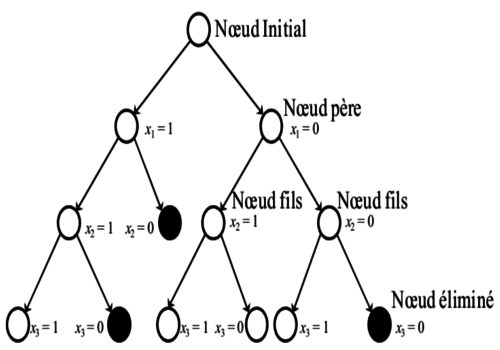
\includegraphics[scale=0.6]{fig1}
  \caption{\label{fig1} Arbre engendr\'e par d\'ecomposition d'un probl\`eme}
  \end{center}
  \end{figure}
%%%%%%%%%%%%%%%%%%%%%%%%%%%%%%%%%%%%%%%%%%%%%%%%%%%%%%%%%%%%%%%%%%%%%%%%%%%%%%%%%%%%%%%%%%%%%%%%%%%%%%%%%%%%%%%%%%%%%%%%%%%%%%%%%%%%%%%%%%%%%%%%%%%%%%%%
%%%%%%%%%%%%%%%%%%%%%%%%%%%%%%%%%%%%%%%%%%%%%%%%%%%%%%%%%%%%%%%%%%%%%%%%%%%%%%%%%%%%%%%%%%%%%%%%%%%%%%%%%%%%%%%%%%%%%%%%%%%%%%%%%%%%%%%%%%%%%%%%%%%%%%%%
\subsection{Methode des coupes planes ou cutting planes m\'ethod}
L\'ethode des coupes \`a \'et\'e d\'evelopp\'ee par A. Schrijver dans son livre intitul\'e {\ Theory of linear and integer programming} en 1986 mais 
les travaux Ralph Edward Gomory ont rendu les cpues plus connues et plus efficaces. Elle est destin\'ee \`a r\'esoudre des probl\`emes d'optimisation
lin\'eaires en nombres entiers qui se formulent sous la forme standard d'un progrmamme lin\'eaire $(PL)$:\\
\begin{equation}
    (PL)  \left\{\begin{array}{l}
               \min C^T x  \\
               s.c.         \\
               Ax \geq b     \\
               x\in \mathbb{R}^n
              \end{array}
      \right.
\end{equation}
L'algorithme de cutting-plane forme une des classes des Algorithmes pour r\'esoudre des PLE's qui utilise une id\'ee sophistiqu\'ee tr\'es
int\'eressante. A chaque \'etape, on diminue la r\'egion r\'ealisable en utilisant un plan coupant (cutting plane) jusqu'\`a ce que la solution 
optimale du PL ({\bfseries relaxation} du PLE) soit enti\`ere correspondant la solution optimale du PLE inital.
{\bf Id\'ee de base: }\\
On ajoute des contraintes lin\'eaires au $PLE$ qui n'excluent pas la solution enti\`ere r\'ealisable.
{\bf Strat\'egie:}
\begin{enumerate}
 \item On ajoute des contraintes lin\'eaires au $PLE$ et donc auussi \`a la relaxation, une \`a chaque \'etape, jusqu'\`a la soluton optimale 
  enti\`ere de la relaxation.
 \item Puis qu'aucune solution r\'ealisable du $PLE$ n'est perdue par les coupes, alors la solution optimale enti\`ere de la relaxation du $PLE$ ayant
 des contrintes ajout\'ees correspondra \`a la solution du $PLE$ d'origine.
\end{enumerate}
 {\bf Observation:}\\
 Consid\'erons un progrmamme en nombres entiers sous la forme standard
 \begin{equation}
  PLE(I) \left\{\begin{array}{l}
                \min  c^Tx  \\
                s.c.         \\
                Ax = b        \\
                x \in \mathbb{Z}_+^n
               \end{array} 
         \right.
 \end{equation}
En supprimant la contrainte d'int\'egrit\'e du $PLE$, on obtient le $PL$ dit relaxation du $PLE$ inital
 \begin{equation}
 PL(II) \left\{\begin{array}{l}
			    \min  c^Tx  \\
			    s.c.         \\
			    Ax = b        \\
			    x \in \mathbb{R}_+^n
			  \end{array} 
		    \right.
 \end{equation}
 On r\'esout le $PL$ obtenu par la m\'ethode du simplexe (voir section \ref{simplexe}) pour aboutir une solution optimale $x^*$.\\
 Si tous les  $x_i^*$,  avec $i\in\{1,2,\hdots,n\}$,  sont enti\`eres, alors $x^*$ correspond \`a $x'$ la solution optimale du $PLE$, sinon on ajoute 
 encore des contraintes puis on continue le processus ci-haut.
 %%%%%%%%%%%%%%%%%%%%%%%%%%%%%%%%%%%%%%%%%%%%%%%%%%%%%%%%%%%%%%%%%%%%%%%%%%%%%%%%%%%%%%%%%%%%%%%%%%%%%%%%%%%%%%%%
 \begin{remarque}
  La m\'ethode des coupes de Gomory nous permet de r\'esoudre un $PLE$ par usage de la m\'ethode du simplexe, mais son principal inconv\'enient est que 
  pour des probl\`emes raisonnables, l'algorithme peut converger parfois d'une mani\`ere trop lente vers la solution optimale.
 \end{remarque}
 %%%%%%%%%%%%%%%%%%%%%%%%%%%%%%%%%%%%%%%%%%%%%%%%%%%%%%%%%%%%%%%%%%%%%%%%%%%%%%%%%%%%%%%%%%%%%%%%%%%%%%%%%%%%%%%%%%%%%%%%%%%%%%%
 \begin{figure}
  \begin{center}
  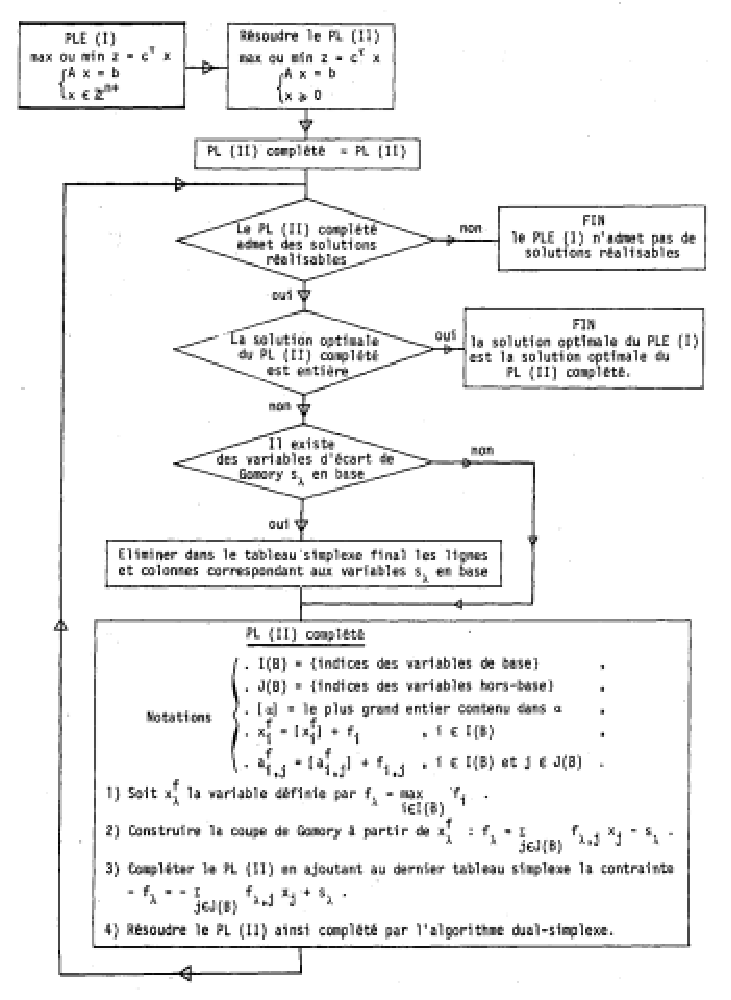
\includegraphics[scale=1.3]{gomory}
  \caption{\label{gomory} Structure de la methode de Gomory, (cf support de cours: Programmation en entiers p.164) }
  \end{center}
\end{figure}
%%%%%%%%%%%%%%%%%%%%%%%%%%%%%%%%%%%%%%%%%%%%%%%%%%%%%%%%%%%%%%%%%%%%%%%%%%%%%%%%%%%%%%%%%%%%%%%%%%%%%%%%%%%%%%%%%%%%%%%%%%%%%%%%%%
%%%%%%%%%%%%%%%%%%%%%%%%%%%%%%%%%%%%%%%%%%%%%%%%%%%%%%%%%%%%%%%%%%%%%%%%%%%%%%%%%%%%%%%%%%%%%%%%%%%%%%%%%%%%%%%%%%%%%%%%%%%%%%%%%%
\subsection{La m\'ethode de Branch \& Cut}
La m\'ethode {\bf Branch \& Cut} est une combinaison de la m\'ethode de Branch and Bound et de la m\'ethode de coupes de Gomory. Cette m\'ethode 
am\'eliore l'inefficacit\'e et le manque de performance de ces deux m\'ethodes face \`a certains probl\`emes appartenant \`a la classe $NP$-difficile.
Pour r\'esoudre un $PLE$, la m\'ethode de {\bf Branch \& Cut} commence d'abord par relaxer le probl\`eme puis appliquer les coupes planes sur la solution
trouv\'ee. Si on obtient une solution non enti\`ere, le probl\`eme sera divis\'e en sous-probl\`emes qui seront r\'esolus de la m\^eme mani\`ere.\\
On se propose de r\'esoudre le probl\`eme d'optimisation suivant par l'algorihme [\ref{alg1}]:
\[(\min c^T x \, : Ax  \geq b ,\, x \in \mathbb{R}^n  ) \]  o\`u  $A\in \mathbb{R}^{m \times n}$ et $b\in \mathbb{R}^n$.
%%%%%%%%%%%%%%%%%%%%%%%%%%%%%% algorihme du B&B %%%%%%%%%%%%%%%%%%%%%%%%%%%%%%%%%%%%%%%%%%%%%%%%%%%%%%%%%%%%%%%%%%%%%%%%%%
\begin{algorithm}
\caption{\textsc{Branch and Cut}}
\label{alg1}
\begin{algorithmic}
\STATE {Liste des probl\`emes  = \emph{vide}}
\REQUIRE {: le programme lin\`eaire par le sous probl\`eme de contraintes\\ $(A_1,b_1)$ avec $A_1 \in \mathbb{R}^{m_1 \times n }$ et 
$b_1 \in \mathbb{R}^{m_1}$ avec $m_1 <<m$;}
\ENSURE{:}
\STATE{Calculer la solution optimale $\bar{x}$ du programme lin\'eaire $c^T \bar{x}=\min (c^T x \, : A_1 x  \geq b_1 ,\, x \in \mathbb{R}^n) $;} 
\STATE{Solution courante = Appliquer la m\'ethode des coupes planes();}
\STATE{\bf Fin \'etapes d'\'evaluation. }\\
\algorithmicif{ la solution courante est r\'ealisable} \algorithmicthen\\
\STATE{$x^* = \bar{x}$ est la solution optimale de $min (c^T x \, : A x  \geq b ,\, x \in \mathbb{R}^n) $; }\\ \algorithmicelse
\STATE{Ajouter le probl\`eme dans Liste des sous probl\`emes;}\\
\algorithmicendif\\
\algorithmicwhile{   Liste des sous probl\`emes $\neq$ \emph{vide} } \algorithmicdo\\
\STATE{S\'electionner un sous probl\`eme;\\ Brancher le probl\`eme; Appliquer les \'etapes d'\'evaluation}\\
\algorithmicendwhile
\end{algorithmic}
\end{algorithm}
%%%%%%%%%%%%%%%%%%%%%%%%%%%%%%%%%%%%%%%%%%%%%%%%%%%%%%%%%%%%%%%%%%%%%%%%%%%%%%%%%%%%%%%%%%%%%%%%%%%%%%%%%%%%%%%%%%%%%%%%%%%%%%%%%%%%%%%%%
\subsection*{Simulation num\'erique de [\ref{alg1}]}
L'algorihme de {\bf Branch and Cut} est utilis\'e dans base du logiciel {\bf IBM(R) ILOG(R) CPLEX(R) optimizer version 12.5.0.0}
comme on va le voir sur le travail pratique suivant:
\[
(PL) \left\{\begin{array}{l}
         \max ( 20x_1 + 8x_2 + 6x_3 + 5x_4 + 4x_5 x_6)\\
         s.c.  \\
         9x_1 + 8x_2 + 6x_3 + 5x_4 + 4x_5 x_6 \leq 12\\
         x_i \in \{0,1\}\,\, \textnormal{avec} \,\, i\in \{1,2,3,4,5,6\}
        \end{array}
 \right.
\]
%%%%%%%%%%%%%%%%%%%%%%%%%%%%%%%%%%%%%%%%%%%%%%%%%%%%%%%%%%%%%%%%%%%%%%%%%%%%%%%%%%%%%%%%%%%%%%%%%%%%%%%%%%%%%%%%%%%%%%%%%%%%%%%%%%%%%%%%%
On \'ecrit le $PL$ sous l'extension {\bf .lp } voir [\ref{fig2}]
%%%%%%%%%%%%%%%%%%%%%%%%%%%%%%%%%%%%%%%%%%%%%%%%%%%%%%%%%%%%%%%%%%%%%%%%%%%%%%%%%%%%%%%%%%%%%%%%%%%%%%%%%%%%%%%%%%%%%%%%%%%%%%%%%%%%%%%%
  \begin{figure}[]
  \begin{center}
  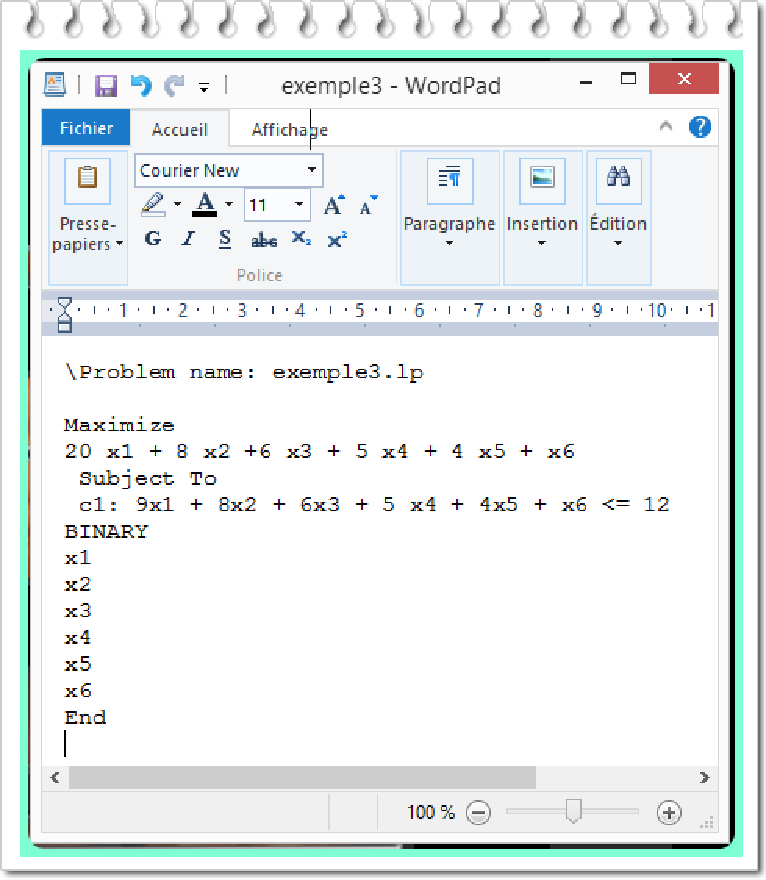
\includegraphics[height=12cm,width=16cm]{formatlp}
  \caption{\label{fig2} Format ``.lp'' du PL comptible au Cplex}
  \end{center}
  \end{figure}
%%%%%%%%%%%%%%%%%%%%%%%%%%%%%%%%%%%%%%%%%%%%%%%%%%%%%%%%%%%%%%%%%%%%%%%%%%%%%%%%%%%%%%%%%%%%%%%%%%%%%%%%%%%%%%%%%%%%%%%%%%%%%%%%%%%%%%%%%
On passe \`a la r\'esolution du $PL$ par le Cplex puis on ontient le r\'esultat suivant sur son terminal:
  \begin{figure}[]
  \begin{center}
  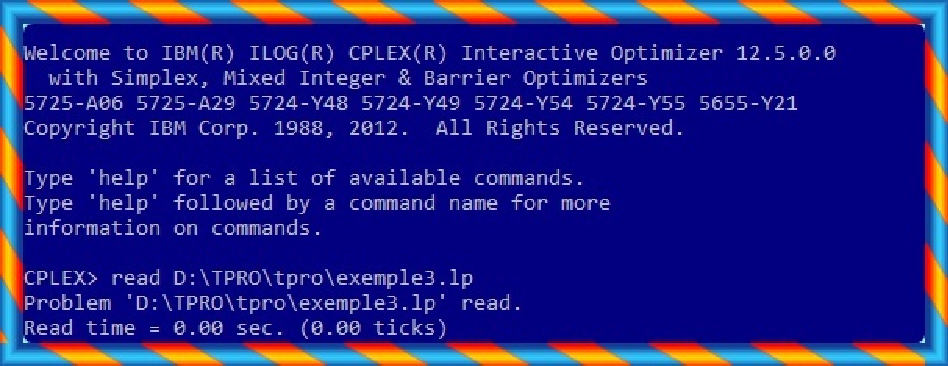
\includegraphics[height=7cm,width=16cm]{tp1}
  \caption{\label{fig2}Leture du PL au format ``.lp'' par Cplex.}
  \end{center}
  \end{figure}
%%%%%%%%%%%%%%%%%%%%%%%%%%%%%%%%%%%%%%%%%%%%%%%%%%%%%%%%%%%%%%%%%%%%%%%%%%%%%%%%%%%%%%%%%%%%%%%%%%%%%%%%%%%%%%%%%%%%%%%%%%%%%%%%%%%%%
 \begin{figure}[]
  \begin{center}
  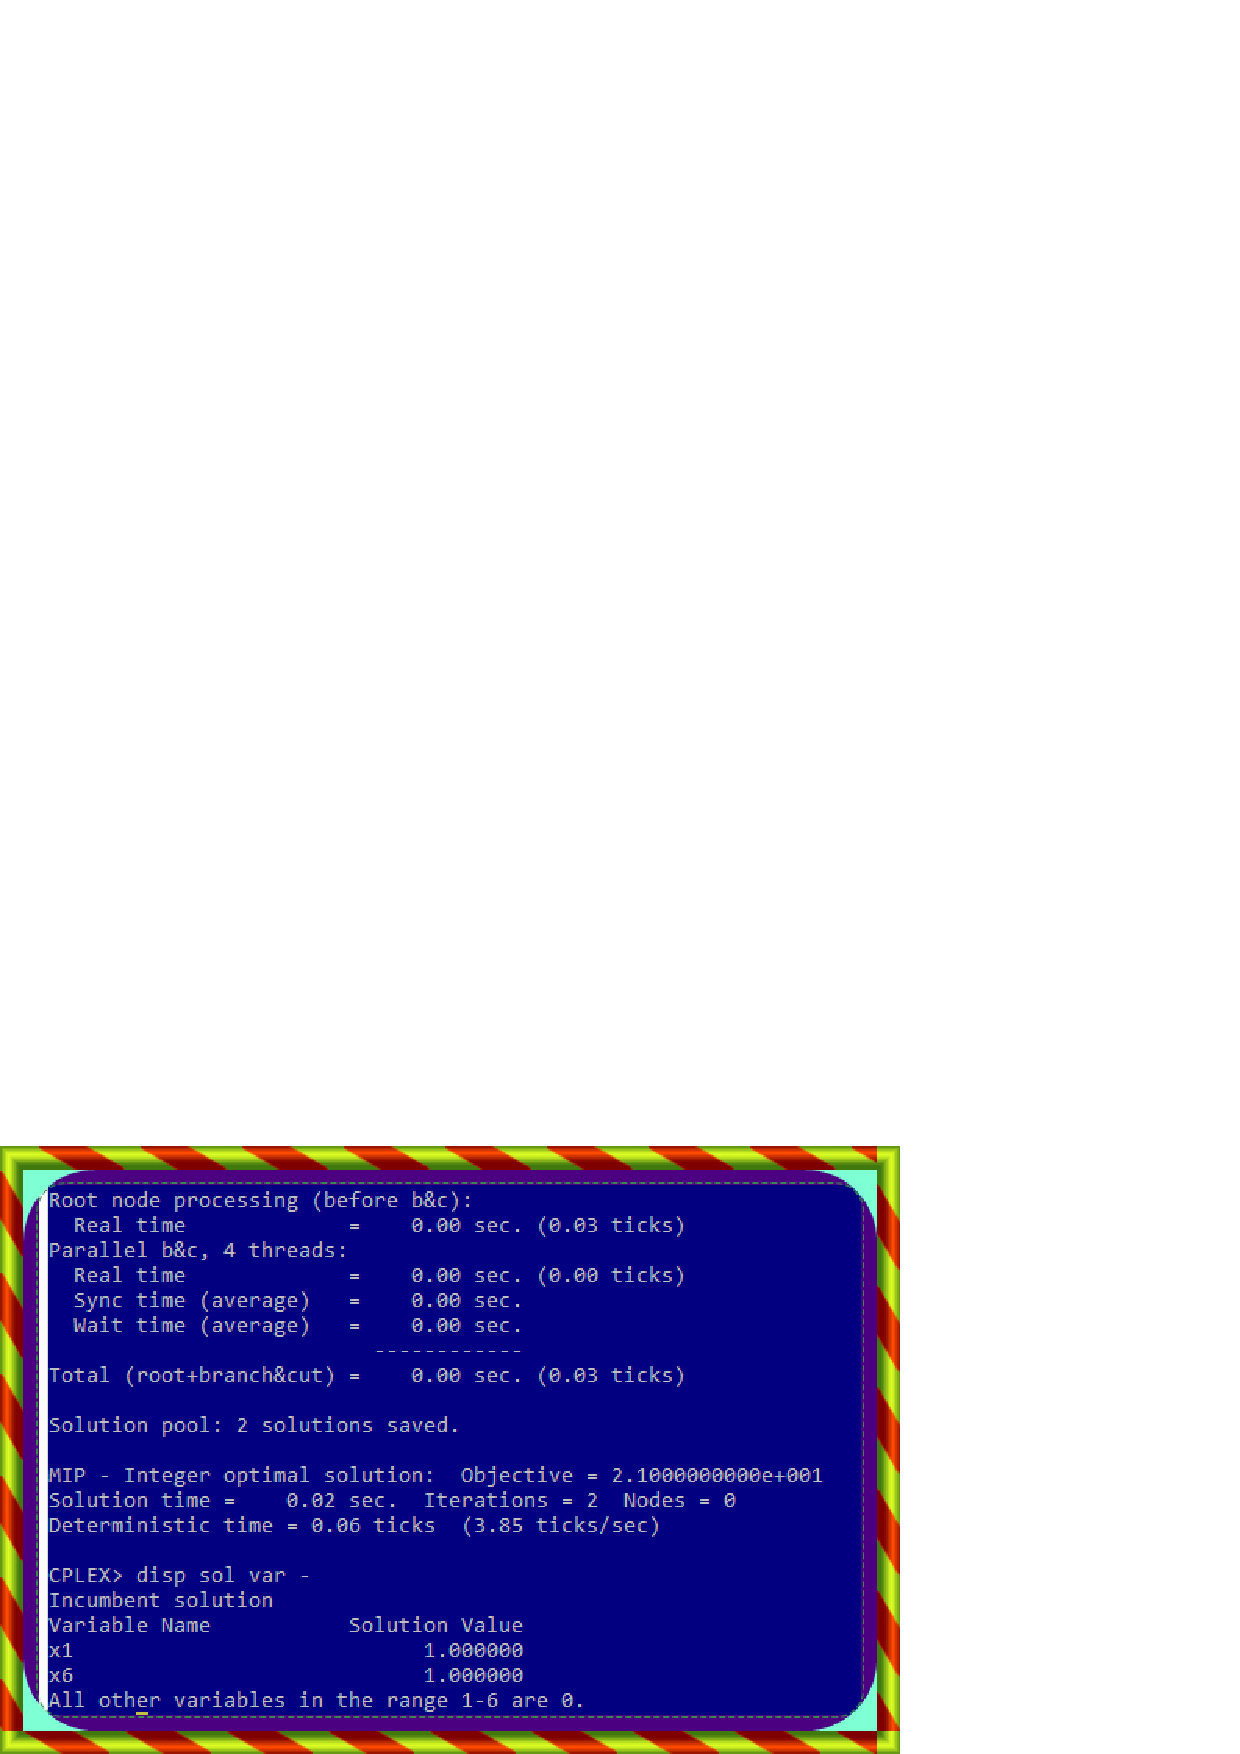
\includegraphics[height=8cm,width=15cm]{tp2}
  \caption{\label{fig2} Details de r\'esolution et affichage du r\'esultat.}
  \end{center}
  \end{figure}
%%%%%%%%%%%%%%%%%%%%%%%%%%%%%%%%%%%%%%%%%%%%%%%%%%%%%%%%%%%%%%%%%%%%%%%%%%%%%%%%%%%%%%%%%%%%%%%%%%%%%%%%%%%%%%%%%%%%%%%%%%%%%%%%%
\begin{remarque}
Il \'existe bien d'autres m\'ethodes de r\'esolution \'exactes des probl\`emes d'optimisation comme la Programmation dynamique, la m\'ethde 
de r\'esolution par Colonies etc. A ce groupe s'ajoute les methodes heuristiques que nous allons voir en d\'etails dans la section suivante.
\end{remarque}
%%%%%%%%%%%%%%%%%%%%%%%%%%%%%%%%%%%%%%%%%%%%%%%%%%%%%%%%%%%%%%%%%%%%%%%%%%%%%%%%%%%%%%%%%%%%%%%%%%%%%%%%%%%%%%%%%%%%%%%%%%%%%%%
\section{Les heuristiques}
En Optimisation combinatoire, une {\bf heuristique} est un algorihme d'approximaton qui permet d'identifier en temps polynomial au moins une 
une solution r\'ealisable rapide, mais obligatoirement optimale. L'usage d'une heuristique est efficace pour Calculer une solution approch\'ee
 d'un probl\`eme et ainsi acc\'el\'erer le processus de r\'esolution \'exacte. G\'en\'eralement une heuristique est con\c{c}ue pour un probl\`eme
 particulier en s'appuyant sur sa structure propre sans offrir aucune garantie quant \`a la qualit\'e de la solution Calcul\'ee. On distingue deux 
 cat\'egories d'heuristiques:
 \begin{description}
  \item[\ding{247}] M\'ethodes constuctives qui g\'en\`erent des solutions \`a partir d'une solution initiale en essayant d'en ajouter petit \`a petit 
  des \'el\'ements jusqu'\`a ce qu'une solution compl\`ete soit obtenue.
  \item[\ding{247}] M\'ethodes de fouilles locales qui d\'emarrent avec solution initialement compl\`ete (probablement moins int\'eressante) et de mani\`ere 
  r\'ep\'etitive essaient d'am\'eliorer cette solution en explorant son voisinage.
 \end{description}
\subsection*{La descente recursive (ou de recherche locale)}
La m\'ethode de descente est l'une des heuristiques les lpus connues. C'est un exemple typique de recherche locale, elle progresse \`a travers l'ensemble 
des solutions $X$ par le choix de la meilleure solution voisinage de la courante et ainsi de suite; ce processus s'interrompt d\'es que le premier minimum 
local est atteint.\\
Cette heuristique est caract\'eris\'ee par sa simplicit\'e mais pr\'esente deux inconv\'enients:
\begin{description}
 \item[\ding{245}] Suivant la taille et la structure du voisinage $N(s)$ consid\'er\'e, la recherche de la meilleure solution voisine qui peut \^etre 
 aussi difficile que le probl\`eme initial.
 \item[\ding{245}] Elle est incapable de progresser au del\`a du premier minimum local rencontr\'e. Par contre les probl\`emes d'optimisation combinatoires
  comportent en g\'en\'erale plusieurs optima locaux pour lesquels la valeur de la fonction objectif peut \^etre fort \'eloign\'ee.
\end{description}





%%%%%%%%%%%%%%%%%%%%%%%%%%%%%%%%%%%%%%%%%%%%%%%%%%%%%%%%%%%%%%%%%%%%%%%%%%%%%%%%%%%%%%%%%%%%%%%%%%%%%%%%%%%%%%%%%%%%%%%%%%%%%%%%%%%%%%%%%%%
\section{Limites}



%%%%%%%%%%%%%%%%%%%%%%%%%%%%%%%%%%%%%%%%%%%%%%%%%%%%%%%%%%%%%%%%%%%%%%%%%%%%%%%%%%%%%%%%%%%%%%%%%%%%%%%%%%%%%%%%%%%%%%%%%%%%%%%%%%%%%%%%%%%%
\section{Conclusion}


%%%%%%%%%%%%%%%%%%%%%%%%%%%%%%%%%%%%%%%%%%%%%%%%%%%%%%%%%%%%%%%%%%%%%%%%
%%%%%%%%%%%%%%%%%%%%%%%%%%%%%%%%%%%%%%%%%%%%%%%%%%%%%%%%%%%%%%%%%%%%%%%%%%
\chapter{Les m\'etaheuristiques}


\subsection{Introduction}
 
\subsection{M\'ethodes \`a base de populations}

\subsubsection{Colonies des fourmis}

\subsubsection{Les algo-g\'en\'etiques}

\subsection{Methodes simples}

\subsubsection{Recuit simil\'e}

\subsubsection{Metroplis}

\subsection{conclusion}

%%%%%%%%%%%%%%%%%%%%%%%%%%%%%%%%%%%%%%%%%%%%%%%%%%%%%%%%%%%%%%%%%%%%%%%%%%%%%%%%%%%
%%%%%%%%%%%%%%%%%%%%%%%%%%%%%%%%%%%%%%%%%%%%%%%%%%%%%%%%%%%%%%%%%%%%%%%%%%%%%%%%%%%
\chapter{Exemples pratiques d'applications}
\minitoc
\subsection{Introduction}

\subsection{Example 1}

\subsection{Example 2}

\subsection{Example 3}

\subsection{conclusion}

\chapter*{Conclusion g\'en\'erale}
\addstarredchapter{Conclusion}




%%%%%%%%%%%%%%%%%%%%%%%%%%%%%%%%%%%%%%%%%%%%%%%%%%%%%%%%%%%%%%%%%%%%%%%%%%%%%%%%%%%%%%%%
\bibliographystyle{unsrt}
\begin{thebibliography}{10}
\mark{References}
\addcontentsline{toc}{chapter}{References}
\addstarredchapter{Bibliographie}

%%%%%%%%%%%%%%%%%%%%%%%%%%%%%%%%%%%%%%%%%%%%%%%%%%%%%%%%%%%%%%%%%%%%%%%%%%%%%%%%%%%%%%%%%%%%%%%%
\bibitem{acherga}
Acher J. ; Gadelle J : 
\emph{Programmation Lin\'eare.} 
Dunod D\'ecision, Bordas, Paris, 1978, Troisi\`eme \'edition .
%%%%%%%%%%%%%%%%%%%%%%%%%%%%%%%%%%%%%%%%%%%%%%%%%%%%%%%%%%%%%%%%%%%%%%%%%%%%%%%%%%%%%%%%%%%%
\bibitem{cea}
C\'ea J. : 
\emph{Optimisation th\'eorique et Algorithmes.}
Dunod, Paris, 1971.
%%%%%%%%%%%%%%%%%%%%%%%%%%%%%%%%%%%%%%%%%%%%%%%%%%%%%%%%%%%%%%%%%%%%%%%%%%%%%%%%%%%%%%%%%
\bibitem{minoux}
Minoux M.:
\emph{Programmation lin\'eaire, th\'eorie et algorithmes.}
Dunond, Tomes 1 et 2

%%%%%%%%%%%%%%%%%%%%%%%%%%%%%%%%%%%%%%%%%%%%%%%%%%%%%%%%%%%%%%%%%%%%%%%%%%%%%%%%%%%%%%%%%%%
\bibitem{werra}
Werra D. :
\emph{El\'ements de programmation lin\'eaire avec application aux graphes.}
Presse polytechniques, 1990, Premi\`ere edition.
%%%%%%%%%%%%%%%%%%%%%%%%%%%%%%%%%%%%%%%%%%%%%%%%%%%%%%%%%%%%%%%%%%%%%%%%%%%%%%%%%%%%%%%%%%%%%%%%
\bibitem{mauras}
Maurras Jean F. :
\emph{Programmation lin\'eaire, Complexit\'e: S\'eparation et Optimisation.}
Spinger-Verlag Berlin, Heidelberg, 2002
%%%%%%%%%%%%%%%%%%%%%%%%%%%%%%%%%%%%%%%%%%%%%%%%%%%%%%%%%%%%%%%%%%%%%%%%%%%%%%%%%%%%%%%%%%%%%%%%%%%%%%%%%%%
\bibitem{Schrijver}
Schrijver A. \label{Schrijver}
\emph{Theory of linear and integer programming.}
Wiley and Sons, 1986, (Cit\'e page 6.)
%%%%%%%%%%%%%%%%%%%%%%%%%%%%%%%%%%%%%%%%%%%%%%%%%%%%%%%%%%%%%%%%%%%%%%%%%%%%%%%%%%%%%%%%%%%%%%%%%%%%%%%%%%%%%%%%%
\bibitem{coursc2si}
coursC2SI.pdf \\
\url{http://www.fsr.ac.ma/cours/maths/bernoussi/Cours\%20C2SI.pdf}
%%%%%%%%%%%%%%%%%%%%%%%%%%%%%%%%%%%%%%%%%%%%%%%%%%%%%%%%%%%%%%%%%%%%%%%%%%%%%%%%%%%%%%%%%%%%%%%%%%%%%%%%%%%%%%
\bibitem{ria}
Revue d'Intelligence Artificielle, Vol: No.1999,\\
\url{http://www.info.univ-angers.fr/pub/hao/papers/RIA.pdf}
%%%%%%%%%%%%%%%%%%%%%%%%%%%%%%%%%%%%%%%%%%%%%%%%%%%%%%%%%%%%%%%%%%%%%%%%%%%%%%%%%%%%%%%%%%%%%%%%%%%%%%%%%%%%%%%%
\bibitem{these}
Th\`ese: conception des m\'etaheuristiques d'optimisation,\\
\url{https://tel.archives-ouvertes.fr/tel-01143778/document}
%%%%%%%%%%%%%%%%%%%%%%%%%%%%%%%%%%%%%%%%%%%%%%%%%%%%%%%%%%%%%%%%%%%%%%%%%%%%%%%%%%%%%%%%%%%%%%%%%%%%%%%%%%%%%%%%%%
\bibitem{alami}
THESE de ALAMI,\\
\url{http://homepages.laas.fr/elbaz/These_LALAMI.pdf}
%%%%%%%%%%%%%%%%%%%%%%%%%%%%%%%%%%%%%%%%%%%%%%%%%%%%%%%%%%%%%%%%%%%%%%%%%%%%%%%%%%%%%%%%%%%%%%%%%%%%%%%%%%%%%%%%%%
\bibitem{kp}
Interstices.info: Le probl\`eme de sac \`a dos,\\
\url{https://interstices.info/jcms/c_19213/le-probleme-du-sac-a-dos }
%%%%%%%%%%%%%%%%%%%%%%%%%%%%%%%%%%%%%%%%%%%%%%%%%%%%%%%%%%%%%%%%%%%%%%%%%%%%%%%%%%%%%%%%%%%%%%%%%%%%%%%%%%%%%%%%%%
\bibitem{gomory}
Algorithme de cutting plane Coupe de Gomory - LITA\\
\url{http://www.lita.univ-lorraine.fr/~kratsch/teaching/ro10.ps}
%%%%%%%%%%%%%%%%%%%%%%%%%%%%%%%%%%%%%%%%%%%%%%%%%%%%%%%%%%%%%%%%%%%%%%%%%%%%%%%%%%%%%%%%%%%%%%%%%%%%%%%%%%%%%%%%%%%
\bibitem{cutting}
Integer programming: cutting planes, (\`a partir de la page 301).\\
\url{http://http://web.mit.edu/15.053/www/AMP-Chapter-09.pdf}
%%%%%%%%%%%%%%%%%%%%%%%%%%%%%%%%%%%%%%%%%%%%%%%%%%%%%%%%%%%%%%%%%%%%%%%%%%%%%%%%%%%%%%%%%%%%%%%%%%%%%%%%%%%%%%%%%%
\bibitem{repere}
REPERE2011,\\
\emph{Ressources El\'ectroniques Pour les Etudiants, la Recherche et l'Enseignemen.}\\
Paris, \`a jour le 01/06/2011, disponible sur:\\
\url{http://repere.enssib.fr}
%%%%%%%%%%%%%%%%%%%%%%%%%%%%%%%%%%%%%%%%%%%%%%%%%%%%%%%%%%%%%%%%%%%%%%%%%%%%%%%%%%%%%%%%%%%%%%%%%%%%%%%%%%%%%%%%%%%%
\bibitem{memoire}
Fouad Bekkari,
\emph{[M\'emoire de Magist\`ere]: R\'esolution des probl\`emes difficiles par optimisation distribu\'ee}
UNIVERSITE MOHAMED KHIDER BISKRA, Alg\'erie, 2008.
%%%%%%%%%%%%%%%%%%%%%%%%%%%%%%%%%%%%%%%%%%%%%%%%%%%%%%%%%%%%%%%%%%%%%%%%%%%%%%%%%%%%%%%%%%%%%%%%%%%%%%%%%%%%%%%%%%

\end{thebibliography}

\end{document}







































































































                                                
























